%% %% %% %%
%%
%% Parte B de la práctica
%%
%% %% %% %%

\documentclass[../procedimientos.tex]{subfiles}
\graphicspath{{\subfix{../../images/}}}

\begin{document}
\clearpage
\subsection{Parte B}
\subsubsection{Instrucciones}
Diseñar e implementar un circuito digital que mediante una señal de control 
$C$ pueda seleccionar el tipo de conversión de código: con $C=1$, GRAY a 
BINARIO y con $C=0$, BINARIO a GRAY. El código es de tres bits.
\begin{figure}[H]
  \centering
  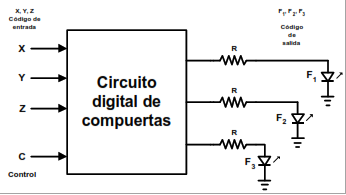
\includegraphics[width=0.5\textwidth]{b_instruction}
  \caption{Ejercicio B}
  \label{fig:b_inst}
\end{figure}

\subsubsection{Análisis}

\subsubsection{Implementación en Quartus}

\end{document}

